%%%%%%%%%%%%%%%%%%%%%%%%%%%%%%%%%%%%%%%%%%%%%%%%
%% Compile the master file!
%% 		Include: Antonio Machicao y Priemer
%% 		Course: GK Linguistik
%%%%%%%%%%%%%%%%%%%%%%%%%%%%%%%%%%%%%%%%%%%%%%%%


%%%%%%%%%%%%%%%%%%%%%%%%%%%%%%%%%%%%%%%%%%%%%%%%%%%%
%%%             Metadata                         
%%%%%%%%%%%%%%%%%%%%%%%%%%%%%%%%%%%%%%%%%%%%%%%%%%%% 

\title{Grundkurs Linguistik}

\subtitle{Graphematik}

\author[A. Machicao y Priemer]{
	{\small Antonio Machicao y Priemer}
	\\
	{\footnotesize \url{http://www.linguistik.hu-berlin.de/staff/amyp}}
	%	\\
	%	{\small\href{mailto:mapriema@hu-berlin.de}{mapriema@hu-berlin.de}}
}

\institute{Institut für deutsche Sprache und Linguistik}

% bitte lassen, sonst kann man nicht sehen, von wann die PDF-Datei ist.
%\date{ }

%\publishers{\textbf{6. linguistischer Methodenworkshop \\ Humboldt-Universität zu Berlin}}

%\hyphenation{nobreak}


%%%%%%%%%%%%%%%%%%%%%%%%%%%%%%%%%%%%%%%%%%%%%%%%%%%%
%%%             Preamble's End                  
%%%%%%%%%%%%%%%%%%%%%%%%%%%%%%%%%%%%%%%%%%%%%%%%%%%%   


%%%%%%%%%%%%%%%%%%%%%%%%%   
\huberlintitlepage[22pt]
\iftoggle{toc}{
	\frame{
		\begin{multicols}{2}
			\frametitle{Inhaltsverzeichnis}
			\tableofcontents
			%[pausesections]
		\end{multicols}
	}
}

%%%%%%%%%%%%%%%%%%%%%%%%%%%%%%%%%%
%%%%%%%%%%%%%%%%%%%%%%%%%%%%%%%%%%
%%%%%LITERATURE:

%% Allgemein
\nocite{Glueck&Roedel16a}
\nocite{Schierholz&Co18}
\nocite{Luedeling2009a}
\nocite{Meibauer&Co07a} 
\nocite{Repp&Co15a} 

%%% Sprache & Sprachwissenschaft
%\nocite{Fries16c} %Adäquatheit
%\nocite{Fries16a} %Grammatikalität
%\nocite{Fries&MyP16c} %GG
%\nocite{Fries&MyP16b} %Akzeptabilität
%\nocite{Fries&MyP16d} %Kompetenz vs. Performanz

%%% Phonetik & Phonologie
%\nocite{Altmann&Co07a}
%\nocite{DudenAussprache00a}
%\nocite{Hall00a} 
%\nocite{Kohler99a}
%\nocite{Krech&Co09a}
%\nocite{Pompino95a}
%\nocite{Ramers08a}
%\nocite{Ramers&Vater92a}
%\nocite{Rues&Co07a}
%\nocite{WieseR96a}
%\nocite{WieseR11a}

%% Graphematik
\nocite{Altmann&Co07a}
\nocite{Duerscheid04a}
\nocite{Eisenberg00a}
\nocite{Fuhrhop08a}
\nocite{Fuhrhop09a}
\nocite{Fuhrhop&Co13a}


%%%%%%%%%%%%%%%%%%%%%%%%%%%%%%%%%%
%%%%%%%%%%%%%%%%%%%%%%%%%%%%%%%%%%
\section{Graphematik}
%%%%%%%%%%%%%%%%%%%%%%%%%%%%%%%%%%


%%%%%%%%%%%%%%%%%%%%%%%%%%%%%%%%%%
\begin{frame}
	\frametitle{Begleitlektüre}
	
	\begin{itemize}
		\item \textbf{obligatorisch:}
		\begin{itemize}
			\item[] AM S.~30--34
			\item[] \citet{Eisenberg04}: Kapitel 8 (S.~301--327)
		\end{itemize}
	\end{itemize}

\end{frame}


%%%%%%%%%%%%%%%%%%%%%%%%%%%%%%%%%%
%%%%%%%%%%%%%%%%%%%%%%%%%%%%%%%%%%
\subsection{Einführung}

%% MyP: Contents
\iftoggle{sectoc}{
	\frame{
		%\begin{multicols}{2}
		\frametitle{~}
		\tableofcontents[currentsubsection, subsubsectionstyle=hide]
		%\end{multicols}
	}
}

%% StM: Contents
\iftoggle{gliederung}{
	
	\outline{
		\begin{itemize}
			
			\item \blaubf{Einführung}
			\item Graph, Graphem, Allograph
			\item Graphematik \vs Orthographie
			\item Schrifttypen \& -systeme
			%%Phonographische Schrifttypen
			%%Logographische Schrifttypen
			%%Fazit: Schrifttypen & -systeme
			%%Tiefe vs. flache Systeme
			\item Graphematische Prinzipien
			%%Phonographisches Prinzip
			%%Silbisches Prinzip
			%%Morphologisches Prinzip
			%%Differenzierung homophoner Formen
			%%Etymologische Schreibung
			%%Ästhetische Schreibung
			%%Syntaktische Schreibung
			\item Hausaufgabe
			
		\end{itemize}
	}
}


%%%%%%%%%%%%%%%%%%%%%%%%%%%%%%%%%%
\begin{frame}
\frametitle{Einführung}

\begin{block}{Graphematik (auch Graphemik)}
	 \textbf{linguistische Teildisziplin}, die sich mit der \textbf{schriftlichen Seite} der Sprache beschäftigt
\end{block}

\pause 

\begin{itemize}

	\item \textbf{Schriftlichkeit} \vs \textbf{Mündlichkeit}
	
	\begin{itemize}
		\item materielle Unterschiede
		\item Unterschied im Gebrauch bzgl.\ Zeitpunkt der Produktion und der Rezeption
		
		\begin{itemize}
			\item  \textbf{Produktion:} 
			
			geschriebener Text benötigt Informationen, die sonst von \textbf{Äußerung oder Kontext} in der gesprochenen Kommunikation gegeben wären.
	
			\item \textbf{Rezeption:} 
			
			geschriebener Text ist \textbf{unabhängig von Zeit und Kontext}.
			
			Einheitlichkeitsregeln werden benötigt, um \textbf{unabhängig verständlich} zu bleiben.
		\end{itemize}

	\end{itemize} 

\end{itemize}

\end{frame}


%%%%%%%%%%%%%%%%%%%%%%%%%%%%%%%%%%
\begin{frame}
\frametitle{Einführung}

\begin{itemize}
	\item Sätze wie (\ref{ex-du-bist-schlau}) und (\ref{ex-nein}) können sehr unterschiedlich gelesen werden.

	\ea\label{ex-du-bist-schlau}
	Du bist schlau.

	\ex\label{ex-nein}
	Nein.
	\z
	
\pause		

\item In der Mündlichkeit vorhandene Informationen: situativer Kontext, Satzintonation, Mimik und Gestik

\item Mögliche \textbf{Kodierung} in der Schriftlichkeit:

	\ea
	DU bist aber \gqq{schlau}!

\begin{multicols}{2}
	\ex 
		\ea nein
		\ex NEIN
		\ex nein!
		\ex nein.
		\ex NEIN.
		\ex *nein
		\z
\end{multicols}

	\z

\end{itemize}		

\end{frame}


%%%%%%%%%%%%%%%%%%%%%%%%%%%%%%%%%%
\begin{frame}
\frametitle{Einführung}

\begin{itemize}
	\item Eine Sprache, \emph{aber} verschiedene \textbf{Varietäten} (Dialekte)
	
	\begin{itemize}
		\item (\idR) eine einzige gemeinsame \textbf{Rechtschreibung}

		\item problemlose Kommunikation über eine bestimmte räumliche Distanz	

	\end{itemize}

\pause

	\item \textbf{Schrift}: ca. 5\,000 Jahre vs. \textbf{Sprache}: ca. 150\,000 Jahre

	\item Man \textbf{lernt} zuerst das Sprechen, bevor man überhaupt schreiben kann und man \textbf{verlernt} eher das Schreiben als das Sprechen.
\end{itemize}

\end{frame}


%%%%%%%%%%%%%%%%%%%%%%%%%%%%%%%%%%
\begin{frame}
\frametitle{Einführung}

\begin{itemize}
	 \item Schriftlichkeit \ras \textbf{System} mit Inventar von Minimaleinheiten und (mehr oder weniger) vorhersagbaren Regeln

	 \item Graphematik \vs Orthographie
	 
	 \begin{itemize}
	 	\item terminologisch manchmal gleich behandelt

	 	\item aber mit unterschiedlichen Zielen, die sie mit unterschiedlichen Methoden verfolgen
	 \end{itemize}
\end{itemize}

\end{frame}


%%%%%%%%%%%%%%%%%%%%%%%%%%%%%%%%%%
%%%%%%%%%%%%%%%%%%%%%%%%%%%%%%%%%%
\subsection{Graph, Graphem, Allograph}

%% MyP: Contents
\iftoggle{sectoc}{
	\frame{
		%\begin{multicols}{2}
		\frametitle{~}
		\tableofcontents[currentsubsection, subsubsectionstyle=hide]
		%\end{multicols}
	}
}

%% StM: Contents
\iftoggle{gliederung}{
	
	\outline{
		\begin{itemize}
			
			\item Einführung
			\item \blaubf{Graph, Graphem, Allograph}
			\item Graphematik \vs Orthographie
			\item Schrifttypen \& -systeme
			%%Phonographische Schrifttypen
			%%Logographische Schrifttypen
			%%Fazit: Schrifttypen & -systeme
			%%Tiefe vs. flache Systeme
			\item Graphematische Prinzipien
			%%Phonographisches Prinzip
			%%Silbisches Prinzip
			%%Morphologisches Prinzip
			%%Differenzierung homophoner Formen
			%%Etymologische Schreibung
			%%Ästhetische Schreibung
			%%Syntaktische Schreibung
			\item Hausaufgabe
			
		\end{itemize}
	}
}


%%%%%%%%%%%%%%%%%%%%%%%%%%%%%%%%%%
\begin{frame}
\frametitle{Graph, Graphem, Allograph}

\begin{itemize}
	\item Graphem: \textbf{Minimaleinheit} der Graphematik

	\item Analog zum Phonembegriff in der Phonologie
\end{itemize}

\begin{block}{Graphem}
kleinste bedeutungsunterscheidende Einheit des Schriftsystems
\end{block}

\pause 

\begin{itemize}
	\item Grapheme sollten \textbf{nicht mit Buchstaben verwechselt werden}.

	\ea \emph{Schwan} besteht aus 6 Buchstaben, aber aus 4 Graphemen.
	\z 
	 	
	\item Grapheme sind \textbf{abstrakte} und \textbf{funktionale} Einheiten,\\
	die durch Buchstaben oder Buchstabenverbindungen realisiert werden können.
\end{itemize}

\end{frame}


%%%%%%%%%%%%%%%%%%%%%%%%%%%%%%%%%%
\begin{frame}
\frametitle{Graph, Graphem, Allograph}

\begin{itemize}
	\item Grapheme kann man, wie auch die Phoneme, durch \textbf{Minimalpaare} ermitteln.
	
	\pause
	 
\settowidth\jamwidth{XXXXXXXXXXXXXXXXXXXXXXXXXXXXXXXX} 

	\ea \ab{war\alertred{d}} \vs \ab{war\alertred{t}} 
	\jambox{
		\only<3->{\ras \ab{d} \vs \ab{t}}
	}
	
	\ex \ab{w\alertred{a}rt} \vs \ab{w\alertred{o}rt} 
	\jambox{
		\only<3->{\ras \ab{a} \vs \ab{o} }
	}
	
	\ex \ab{\alertred{w}art} \vs \ab{\alertred{p}art} 
	\jambox{
		\only<3->{\ras \ab{w} \vs \ab{p} }
	}
	
	\ex \ab{pa\alertred{r}t} \vs \ab{pa\alertred{ch}t} 
	\jambox{
		\only<3->{\ras \ab{r} \vs \ab{ch} }
	}
	\z
\end{itemize}

\end{frame}


%%%%%%%%%%%%%%%%%%%%%%%%%%%%%%%%%%
\begin{frame}
\frametitle{Graph, Graphem, Allograph}

	\begin{itemize}
		\item \textbf{Graph}: tatsächliche Realisierung eines Graphems
		\item \textbf{Allographe}: unterschiedliche Graphe, die mögliche Realisierung eines Graphems sind
		\item[]
		\item Ein Graph, ein Allograph und ein Graphem notiert man\\
		mit den spitzen Klammern \ab{}.
	
		\ea Graphem: \ab{a}

		\ex	Allographe von \ab{a}: \ab{\textit{a}} \ab{\textswab{a}} \ab{a} \ab{\textfrak{a}} \ab{{\Large \calligra{a}}\,} \ab{\texttt{a}}
		\z 
		
		\item In einigen älteren Arbeiten unterscheidet man die Notation von Graphemen \ab{a} in einfachen spitzen Klammern von der Notation von Graphen $\langle \langle$a$\rangle \rangle$ in doppelten spitzen Klammern.
	\end{itemize}


\end{frame}


%%%%%%%%%%%%%%%%%%%%%%%%%%%%%%%%%%
%%%%%%%%%%%%%%%%%%%%%%%%%%%%%%%%%%
\subsection{Graphematik \vs Orthographie}

%% MyP: Contents
\iftoggle{sectoc}{
	\frame{
		%\begin{multicols}{2}
		\frametitle{~}
		\tableofcontents[currentsubsection, subsubsectionstyle=hide]
		%\end{multicols}
	}
}

%% StM: Contents
\iftoggle{gliederung}{
	
	\outline{
		\begin{itemize}
			
			\item Einführung
			\item Graph, Graphem, Allograph
			\item \blaubf{Graphematik \vs Orthographie}
			\item Schrifttypen \& -systeme
			%%Phonographische Schrifttypen
			%%Logographische Schrifttypen
			%%Fazit: Schrifttypen & -systeme
			%%Tiefe vs. flache Systeme
			\item Graphematische Prinzipien
			%%Phonographisches Prinzip
			%%Silbisches Prinzip
			%%Morphologisches Prinzip
			%%Differenzierung homophoner Formen
			%%Etymologische Schreibung
			%%Ästhetische Schreibung
			%%Syntaktische Schreibung
			\item Hausaufgabe
			
		\end{itemize}
	}
}


%%%%%%%%%%%%%%%%%%%%%%%%%%%%%%%%%%
\begin{frame}
\frametitle{Graphematik \vs Orthographie}

	\begin{itemize}
		\item Die Graphematik ist ein \textbf{Teilbereich der Linguistik}, der sich mit dem (\textbf{unabhängigen} und \textbf{natürlichen}) \textbf{Schriftsystem} befasst.
		
		\begin{itemize}
			\item Hauptaufgabe: \textbf{Erklären}, warum Wörter und Sätze (und darüber hinaus auch Texte) so geschrieben werden
			\item Notwendig: \textbf{Regelmäßigkeiten} und Prinzipien, die dem normalen Schreiben zugrunde liegen
			\item Empirische Basis: Schreibusus
		\end{itemize}
			
		\item Graphematisches System \ras \textbf{natürliches System} (wie das phonologische oder syntaktische System)
		\item ABER:
		
		\begin{itemize}
			\item Erlernen der Schriftsprache \ras \textbf{explizit} und angelehnt an Norm
			\item Erlernen der mündlichen (Erst-)Sprache \ras \textbf{natürlich}	
		\end{itemize}
	\end{itemize}
\end{frame}


%%%%%%%%%%%%%%%%%%%%%%%%%%%%%%%%%%
\begin{frame}
\frametitle{Graphematik \vs Orthographie}

\begin{block}{Graphematik}
	Wissenschaft vom \textbf{Schriftsystem einer Sprache}, die die Regularitäten des Schriftsystems auf \textbf{segmentaler} und \textbf{suprasegmentaler} Ebene \textbf{beschreibt}. Diese Regularitäten finden ihre empirische Basis im \textbf{Schreibusus}, \dash darin, wie tatsächlich geschrieben wird \citep[vgl.][140]{Duerscheid04a}.
\end{block}

\end{frame}


%%%%%%%%%%%%%%%%%%%%%%%%%%%%%%%%%%
\begin{frame}
\frametitle{Graphematik \vs Orthographie}

\begin{itemize}
	\item Die Orthographie (Rechtschreibung) ist dagegen eine \textbf{\gqq{willkürliche} Festlegung}. Sie legt fest, was \textbf{\gqq{richtig}} oder \textbf{\gqq{falsch}} (nach einer bestimmten Norm) ist.
	
	\begin{itemize}
		\item Ergebnis der Rechtschreibung: \textbf{explizit geregeltes} und \textbf{per Konventionen akzeptiertes} System
		
		\item Die normative Instanz (Orthographie) resultiert häufig aus \textbf{(sprach-)politischen} Entscheidungen.
		
		\item Das aus der Graphematik explizit gemachte Wissen spielt eine bedeutende Rolle für die Entwicklung der Orthographie.

\pause
		
		\item Graphematik: \textbf{Beschreibung} des Schriftsystems
		
		\item Orthographie: \textbf{Normierung} des Schriftsystems
	\end{itemize}
\end{itemize}

\end{frame}


%%%%%%%%%%%%%%%%%%%%%%%%%%%%%%%%%%
\begin{frame}{Graphematik \vs Orthographie}

\begin{block}{Orthographie}
	Disziplin, die das \textbf{Regelsystem}, das dem Schreiber als \textbf{externe Normen} vorgegeben wird, entwickelt. Die normativen Festlegungen basieren \idR auf den in der Graphematik gewonnenen Erkenntnissen \citep[vgl.][141]{Duerscheid04a}.
\end{block}

\end{frame}


%%%%%%%%%%%%%%%%%%%%%%%%%%%%%%%%%%
\begin{frame}
\frametitle{Graphematik \vs Orthographie}

%\begin{itemize}
%	\item[]

Wie wird das Wort \textipa{[\textscr a:t]} geschrieben?

        \pause
	\begin{table}
		\centering
		%\scalebox{0.9}{
		\begin{tabular}{l | c | l}
			\ab{R\alertred{ah}t}, \ab{R\alertred{ah}d} & ah & vgl. \ab{Kahn}\\ 
			\hline
			\ab{R\alertred{aa}d}, \ab{R\alertred{aa}t} & aa & vgl. \ab{Aal}\\ 
			\hline
			\ab{R\alertred{ar}d}, \ab{R\alertred{ar}t} & ar & vgl. \ab{Bart} als \textipa{[ba:t]}\\ 
			\hline
			\ab{R\alertred{ahr}t} & ahr	& vgl. \ab{Fahrt} als \textipa{[fa:t]}\\
			\hline
			\ab{Ra\alertred{d}} & d & vgl. \ab{Bad}\\ 
			\hline
			\ab{Ra\alertred{t}} & t & vgl. \ab{Tat}\\ 
		\end{tabular} 
		%}
	\end{table}

%\end{itemize}
\end{frame}



%%%%%%%%%%%%%%%%%%%%%%%%%%%%%%%%%%
\begin{frame}
\frametitle{Graphematik \vs Orthographie}

\begin{itemize}
	\item \textbf{Graphematisch} sind unterschiedliche Schreibungen möglich.

\pause 
	
	\item \textbf{Orthographisch} gibt es \textbf{nur zwei richtige} Schreibungen: \\
	\ab{Rad} oder \ab{Rat}
	\item[]
	\item Gleiche Lautung, aber verschiedene \gqq{Wörter}
	
	\begin{itemize}
		\item \textbf{Morphemkonstanz} (\su): \ab{Rad} wird mit \ab{d} geschrieben, um die \textbf{morphologische Verwandtschaft} zu anderen Wortformen im Paradigma anzuzeigen.
		
		\ea \ab{Räder}, \ab{Rädern}, \ab{radeln}
		\z 

		\item \textbf{Homonymiedifferenzierung} (\su): Zwei Wörter mit der \textbf{gleichen Lautung, aber verschiedenen Bedeutungen,} sollten möglichst verschieden geschrieben werden.
		
		\begin{itemize}
			\item Unterschiedliche Bedeutungen können anhand der Schrift, aber nicht der Lautung, differenziert werden!
		\end{itemize}
	\end{itemize}
\end{itemize}

\end{frame}


%%%%%%%%%%%%%%%%%%%%%%%%%%%%%%%%%%
\begin{frame}
\frametitle{Graphematik \vs Orthographie}

\begin{itemize}
	\item Die Orthographie legt \idR eine einzige, \textbf{verbindliche Form} für die Schreibung eines Wortes fest.
	
	\begin{itemize}
		\item Orthographische Normierung: möglichst \textbf{geringe Variabilität} in der Schreibung

\pause

		\item Weniger als 1\% der Wörter variabel
			
		\ea Graphik/Grafik, Cousine/Kusine, Friseur/Frisör, Nougat/Nugat, so dass/sodass, mithilfe/mit Hilfe, Orthographie/Orthografie \dots
		\z

\pause 
			
		\item Abweichungen in der Schreibung können auch auf internen, \textbf{nicht-kodifizierten} Normen beruhen.
			
		\ea die Klassiker Bibliothek, Ulla's Lädchen, Hits für Kid's, BahnCard, StudentInnen, Student\_innen, Student*innen\dots
		\z
	\end{itemize}
\end{itemize}

\end{frame}


%%%%%%%%%%%%%%%%%%%%%%%%%%%%%%%%%%
\begin{frame}
\frametitle{Graphematik \vs Orthographie}

\begin{itemize}
	\item \textbf{Gemeinsames Ziel} von Graphematik und Orthographie:\\
	 Schreiben und Lesen möglichst \textbf{reibungslos} und \textbf{intuitiv} gestalten

	\item Regeln müssen systematisch nachvollziehbar sein:
	
	\ea \ab{fertig} nicht mit \ab{v}, sondern mit \ab{f} 
	
	\ab{fer} in \ab{fertig} hat nicht die gleiche Bedeutung wie \ab{ver} in \ab{verpetzt} oder \ab{verschreiben}
	\z
	
	\item Beschäftigung mit dem \textbf{Erstspracherwerb} bei Kindern und mit der \textbf{Fehleranalyse} ist für die Erstellung der Prinzipien von besonderer Bedeutung.
\end{itemize}

\end{frame}


%%%%%%%%%%%%%%%%%%%%%%%%%%%%%%%%%%
%%%%%%%%%%%%%%%%%%%%%%%%%%%%%%%%%%
\subsection{Schrifttypen \& -systeme}

%% MyP: Contents
\iftoggle{sectoc}{
	\frame{
		%\begin{multicols}{2}
		\frametitle{~}
		\tableofcontents[currentsubsection, subsubsectionstyle=hide]
		%\end{multicols}
	}
}

%% StM: Contents
\iftoggle{gliederung}{
	
	\outline{
		\begin{itemize}
			
			\item Einführung
			\item Graph, Graphem, Allograph
			\item Graphematik \vs Orthographie
			\item \blaubf{Schrifttypen \& -systeme}
			%%Phonographische Schrifttypen
			%%Logographische Schrifttypen
			%%Fazit: Schrifttypen & -systeme
			%%Tiefe vs. flache Systeme
			\item Graphematische Prinzipien
			%%Phonographisches Prinzip
			%%Silbisches Prinzip
			%%Morphologisches Prinzip
			%%Differenzierung homophoner Formen
			%%Etymologische Schreibung
			%%Ästhetische Schreibung
			%%Syntaktische Schreibung
			\item Hausaufgabe
			
		\end{itemize}
	}
}


%%%%%%%%%%%%%%%%%%%%%%%%%%%%%%%%%%
\begin{frame}
\frametitle{Schrifttypen \& -systeme}


\begin{block}{Schriftsystem}
	Regularitäten in der schriftlichen Realisierung einer bestimmten Sprache
\end{block}

\ea \textbf{Das deutsche Schriftsystem} verwendet das Zeichen \gqq{ß}.
\z 

\pause 

\begin{itemize}
	\item Verschiedene Arten von Schriftsystemen gehören zu einem Schrifttyp. 
	
	\ea Das deutsche, das französische und das englische Schriftsystem gehören zu den \textbf{phonographischen Schrifttypen} \\
	(graphische Einheiten (Buchstaben) entsprechen lautlichen Einheiten).
	\z 
\end{itemize}

\begin{block}{Schrifttyp}
	Art der \textbf{Beziehung} zwischen \textbf{sprachlichen} und \textbf{graphischen} Einheiten
\end{block}	

\end{frame}


%%%%%%%%%%%%%%%%%%%%%%%%%%%%%%%%%%%
\begin{frame}
\frametitle{Übersicht der Schrifttypen \& -systeme}


\begin{figure}
	\centering
	\scalebox{.85}{
	\begin{forest}
	MyP edges
	[\textbf{\alertred{Schrifttypen}}
		[\textbf{logographischer} \\ Schrifttyp
			[Chinesisch \\ Hieroglyphen, tier=word]
		]
		[\textbf{phonographischer} \\ Schrifttyp
			[\textbf{alphabetischer} \\ Schrifttyp
				[\textbf{Konsonant-Vokal-}\\Schriften
					[Latein \\ Griechisch \\ Russisch, tier=word]
				]
				[\textbf{Konsonanten-}\\schriften
					[Hebräisch \\ Arabisch, tier=word]
				]
			]
			[\textbf{syllabischer} \\ Schrifttyp
				[Japanisch \\ Koreanisch, tier=word, name=anchor] {
					\node [right=of anchor]{\textbf{\alertred{Schriftsysteme}}};
			}
			]
		]
	]
	\end{forest}
}
\end{figure}

\end{frame}


%%%%%%%%%%%%%%%%%%%%%%%%%%%%%%%%%%
%%%%%%%%%%%%%%%%%%%%%%%%%%%%%%%%%%
\subsubsection{Phonographische Schrifttypen}
%\iftoggle{sectoc}{
%	\frame{
%		\begin{multicols}{2}
%			\frametitle{~}
%			\tableofcontents[currentsection]
%		\end{multicols}
%	}
%}
%%%%%%%%%%%%%%%%%%%%%%%%%%%%%%%%%%

\begin{frame}
\frametitle{Phonographische Schrifttypen}



\begin{itemize}
	\item Grundformen (\zB Grapheme) sind primär auf \textbf{bedeutungsunterscheidende} Elemente (\zB Phoneme in (\ref{ex:DtGraf}) oder Silben (s.\ Abb.)) im Sprachsystem bezogen \citep[vgl.][76--77]{Duerscheid04a}.
\end{itemize}
	 
\hfill 	 
\begin{minipage}{.47\textwidth}
	\ea\label{ex:DtGraf} Deutsch:
	\ab{k} für Laut \textipa{[k]}
	\z 
\end{minipage}%\hfill%
%%
%%
\begin{minipage}{.5\textwidth}
\begin{figure}
	\centering
	
	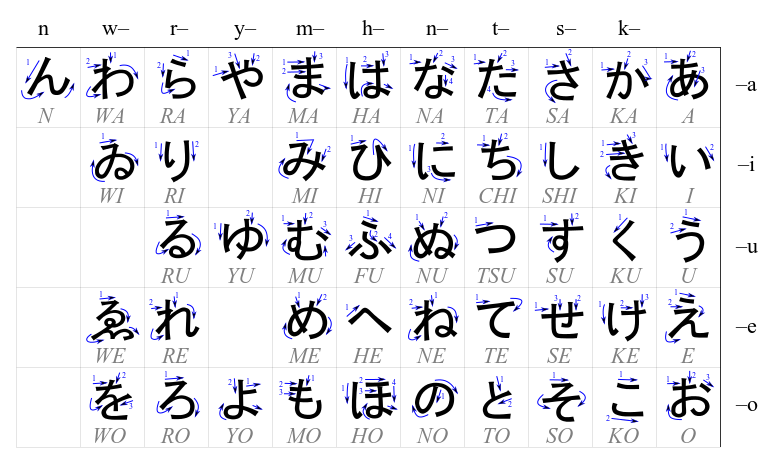
\includegraphics[scale=.2]{material/05Table_hiragana}
	\caption{Hiragana mit lat. Umschrift}
	\label{Hiragana}
\end{figure}
\end{minipage}

\end{frame}


%%%%%%%%%%%%%%%%%%%%%%%%%%%%%%%%%%
\begin{frame}
\frametitle{Phonographische Schrifttypen: Syllabisch}

%\begin{minipage}{.59\textwidth}
\begin{itemize}
	\item Korrespondenz zwischen \textbf{graphischem Zeichen} und \textbf{Silbe}
	\item Japanisch, Koreanisch, \dots
	
	%\ex. Japanisch: [Japanisch Package] für die Silbe \textipa{[ka]} (in der Silbenschrift Hiragana)

\end{itemize}
%\end{minipage}\hfill%
%%
%%
%\begin{minipage}{.4\textwidth}
	\begin{figure}
		\centering
		
		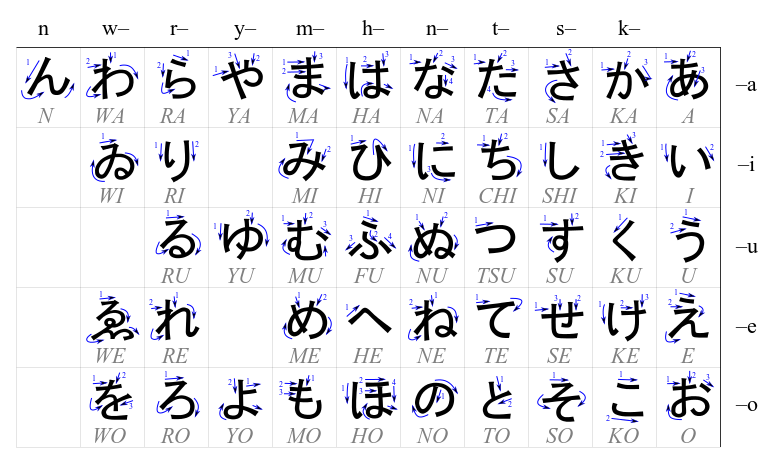
\includegraphics[scale=.25]{material/05Table_hiragana}
		\caption{Hiragana mit lat. Umschrift}
%		\label{Hiragana}
	\end{figure}
%\end{minipage}

\end{frame}


%%%%%%%%%%%%%%%%%%%%%%%%%%%%%%%%%%
\begin{frame}
\frametitle{Phonographische Schrifttypen: Alphabetisch}


\begin{itemize}

	\item Korrespondenz zwischen \textbf{graphischem Zeichen} (Buchstaben) und \textbf{Lauten}
	\item Deutsch, Russisch, Arabisch, \dots
	
	\ea Deutsch: \ab{t} für Laut \textipa{[t]}
	\z 
	
	\pause 
	
	\begin{itemize}
		\item \textbf{Konsonant-Vokal-Schrift:} \\
		enthält Grapheme für Konsonanten und Vokale
		\item Deutsch, Russisch, \dots
		
		\item \textbf{Konsonantenschrift:}\\
		enthält Grapheme (fast) nur für Konsonanten \citep[vgl.][358]{Glueck16b} 
		\item nordwestsemitische Schriftarten, Arabisch, Hebräisch, \dots
	\end{itemize}
	
	\end{itemize}

\end{frame}


%%%%%%%%%%%%%%%%%%%%%%%%%%%%%%%%%%
%%%%%%%%%%%%%%%%%%%%%%%%%%%%%%%%%%
\subsubsection{Logographische Schrifttypen}
%\iftoggle{sectoc}{
%	\frame{
%		\begin{multicols}{2}
%			\frametitle{~}
%			\tableofcontents[currentsection]
%		\end{multicols}
%	}
%}
%%%%%%%%%%%%%%%%%%%%%%%%%%%%%%%%%%

\begin{frame}
\frametitle{Logographische Schrifttypen}

\begin{itemize}
	\item Grundformen sind primär auf \textbf{bedeutungstragende} Elemente (\zB Wörter oder Morpheme) im Sprachsystem bezogen \citep[vgl.][76--77]{Duerscheid04a}. 
	
	\item Chinesisch, Teile der ägyptischen Hieroglyphen
\end{itemize}
		
\begin{minipage}{.28\textwidth}
	\begin{figure}
	\centering
	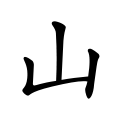
\includegraphics[scale=.45]{material/Chinesemountain-Lee-Sau-Dan}
	\caption[chinese]{Chinesisches Zeichen für `Berg'}\label{ChinBerg}
	\end{figure}
\end{minipage}\hfill%
%%
\begin{minipage}{.68\textwidth}
	\begin{figure}
	\centering
	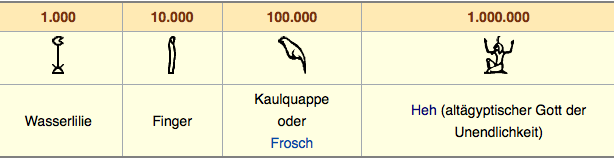
\includegraphics[scale=.37]{material/04Hieroglyphenzahlen}
	\caption[Hiero]{Hieroglyphenzahlen}\label{Hieroglyphen}
	\end{figure}
\end{minipage}
		
\end{frame}


%%%%%%%%%%%%%%%%%%%%%%%%%%%%%%%%%%
%%%%%%%%%%%%%%%%%%%%%%%%%%%%%%%%%%
\subsubsection{Fazit: Schrifttypen \& -systeme}
%\iftoggle{sectoc}{
%	\frame{
%		\begin{multicols}{2}
%			\frametitle{~}
%			\tableofcontents[currentsection]
%		\end{multicols}
%	}
%}
%%%%%%%%%%%%%%%%%%%%%%%%%%%%%%%%%%

\begin{frame}
\frametitle{Fazit: Schrifttypen \& -systeme}

\begin{itemize}
	\item Vorteil von \textbf{phonographischen} Schriftsystemen:
	
	\begin{itemize}
		\item große Menge von Wörtern mit \textbf{eher kleinem Inventar von Zeichen} (20--30) darstellbar
	\end{itemize}
	
	\item \textbf{Logographische Schrifttypen} benötigen sehr viele Zeichen.
	
	\begin{itemize}
		\item Das chinesische Schriftsystem besteht aus ungefähr 87\,000 Zeichen,\\
                  von denen zwischen 3\,000 und 5\,000 für den Alltag benötigt werden.
	\end{itemize}
	
\pause 	

	\item Vorteil von \textbf{logographischen} Schriftsystemen:
	\begin{itemize}
		\item Sie können auch von Lesern anderer Dialekte \textbf{relativ leicht dekodiert} werden.
	\end{itemize}	
\end{itemize}
\end{frame}


%%%%%%%%%%%%%%%%%%%%%%%%%%%%%%%%%%%%
%\begin{frame}
%\frametitle{Übersicht der Schrifttypen \& -systeme}
%
%
%\begin{figure}
%\centering
%\scalebox{.85}{
%	\begin{forest}
%		MyP edges
%		[\textbf{\alertred{Schrifttypen}}
%			[\textbf{logographischer} \\ Schrifttyp
%			[Chinesisch \\ Hieroglyphen, tier=word]
%			]
%			[\textbf{phonographischer} \\ Schrifttyp
%				[\textbf{alphabetischer} \\ Schrifttyp
%					[\textbf{Konsonant-Vokal-}\\Schriften
%						[Latein \\ Griechisch \\ Russisch, tier=word]
%					]
%					[\textbf{Konsonanten-}\\schriften
%						[Hebräisch \\ Arabisch, tier=word]
%					]
%				]
%				[\textbf{syllabischer} \\ Schrifttyp
%					[Japanisch \\ Koreanisch, tier=word, name=anchor] {
%					\node [right=of anchor]{\textbf{\alertred{Schriftsysteme}}};
%					}
%				]
%			]
%		]
%	\end{forest}
%}
%\end{figure}
%
%\end{frame}
%
%
%%%%%%%%%%%%%%%%%%%%%%%%%%%%%%%%%%
%%%%%%%%%%%%%%%%%%%%%%%%%%%%%%%%%%
\subsubsection{Tiefe \vs flache Systeme}
%\iftoggle{sectoc}{
%	\frame{
%		\begin{multicols}{2}
%			\frametitle{~}
%			\tableofcontents[currentsection]
%		\end{multicols}
%	}
%}
%%%%%%%%%%%%%%%%%%%%%%%%%%%%%%%%%%

\begin{frame}
\frametitle{Tiefe vs.\ flache Systeme}

\begin{itemize}
	\item trotz phonographischer/""alphabetischer Schriftsysteme \ras\\
              sehr verschiedene Schreibung in den unterschiedlichen Sprachen

	\item unterschiedliche \textbf{graphematische (/orthographische) Prinzipien},\\
          die den unterschiedlichen Schreibungen zugrunde liegen

	\item Selten 1-zu-1-Korrespondenz zwischen Phonemen und Graphemen
	
	\begin{itemize}
		\item \textbf{tiefes System}\\ 
		\vs
		\item \textbf{flaches System}
	\end{itemize}
\end{itemize}
\end{frame}


%%%%%%%%%%%%%%%%%%%%%%%%%%%%%%%%%%
\begin{frame}
\frametitle{Tiefe vs.\ flache Systeme}
\begin{itemize}
	
	\item \textbf{flaches System:}

	\begin{itemize}
		
		\item sehr gute 1-zu-1-Abbildung von Phonemen und Graphemen
		
		\item \textbf{Türkisch}
		
		\begin{itemize}
			
			\item 1928: Ersetzung der arabischen Schrift durch die lateinische Schrift
			
			\item besonders gute Phonem-Graphem-Abbildung
		\end{itemize}
	\end{itemize}

\pause 

	\item \textbf{tiefes System:}

\begin{itemize}

	\item Abbildung von Phonemen auf Graphemen, aber mit Einschränkung

	\item \textbf{Englisch} oder \textbf{Französisch}
	
	\begin{itemize}
		\item nicht häufig \textbf{reformiert} \ras starke Abweichung von Aussprache und Schriftform

		\item Englisch: \textbf{altes} und \textbf{gewachsenes} System mit sehr verschiedenen \textbf{Dialekten} in unterschiedlichen Ländern

		\item schriftliche Verständigung zwischen den Varietäten ist nur gewährleistet,\\
		wenn die Phonem-Graphem-Korrespondenz nicht streng durchgezogen wird.
	\end{itemize}
\end{itemize}
\end{itemize}

\end{frame}


%%%%%%%%%%%%%%%%%%%%%%%%%%%%%%%%%%
\begin{frame}
\frametitle{Tiefe vs.\ flache Systeme}


	\ea Türkisch: \\
	\ab{dükkan} für \textipa{[dYkkan]}
	
	\ex Spanisch: \\
	\ab{negocio} für \textipa{[negoTio]}
	
	\ex Englisch: \\
	\ab{business} für \textipa{[bIzn@z]}
	
	\ex Französisch: \\
	\ab{boutique} für \textipa{[butik]}
	\z 
	
\pause	
	
	\ea English: \ab{gh o ti} für \ab{fish} 

\pause  
	
	(\ab{gh} wie in \ab{enou\alertred{gh}}, \ab{o} wie in \ab{w\alertred{o}men}, \ab{ti} wie in \ab{na\alertred{ti}on}
	\z 

\end{frame}


%%%%%%%%%%%%%%%%%%%%%%%%%%%%%%%%%%
\begin{frame}
\frametitle{Tiefe vs.\ flache Systeme}


\begin{figure}
\centering
	
\includegraphics[scale=.3]{material/04GraphEnglischPGK}
	\caption{Englisch und PGK}\label{grammarlycard}
%{https://www.facebook.com/grammarly/photos/a.158139670871698.33824.139729956046003/942699349082389/; Autor: Grammarly; Stand: 05.12.16}
\end{figure}

\end{frame}


%%%%%%%%%%%%%%%%%%%%%%%%%%%%%%%%%%
%%%%%%%%%%%%%%%%%%%%%%%%%%%%%%%%%%
\subsection{Graphematische Prinzipien}

%% MyP: Contents
\iftoggle{sectoc}{
	\frame{
		%\begin{multicols}{2}
		\frametitle{~}
		\tableofcontents[currentsubsection, subsubsectionstyle=hide]
		%\end{multicols}
	}
}

%% StM: Contents
\iftoggle{gliederung}{
	
	\outline{
		\begin{itemize}
			
			\item Einführung
			\item Graph, Graphem, Allograph
			\item Graphematik \vs Orthographie
			\item Schrifttypen \& -systeme
			%%Phonographische Schrifttypen
			%%Logographische Schrifttypen
			%%Fazit: Schrifttypen & -systeme
			%%Tiefe vs. flache Systeme
			\item \blaubf{Graphematische Prinzipien}
			%%Phonographisches Prinzip
			%%Silbisches Prinzip
			%%Morphologisches Prinzip
			%%Differenzierung homophoner Formen
			%%Etymologische Schreibung
			%%Ästhetische Schreibung
			%%Syntaktische Schreibung
			\item Hausaufgabe
			
		\end{itemize}
	}
}


%%%%%%%%%%%%%%%%%%%%%%%%%%%%%%%%%%
\begin{frame}
\frametitle{Graphematische Prinzipien/Tendenzen}

\begin{itemize}
	\item \textbf{Schrifttyp} bedingt das graphematische System.
	\item Daraus ergibt sich die \textbf{Gewichtung} (oder Vorhandensein) weiterer
Prinzipien:

	\begin{itemize}
		\item Deutsch: alphabetischer Schrifttyp \ras Abbildung von Phonemen mit Graphemen

		\item Abbildung von Phonemen auf Grapheme $=$ \\
		\textbf{Phonem-Graphem-Korrespondenz} (PGK)
		
		\item Weitere Prinzipien:
		
		\begin{itemize}
			\item \textbf{Wortebene}:\\
			regelhafte Markierung von Silben, Morphemen und Bedeutungseinheiten, \dots

			\item \textbf{Satzebene}: \\
			regelhafte Groß- und Kleinschreibung, Zusammen- und Getrenntschreibung, \dots
		\end{itemize}
	
	\end{itemize}

\end{itemize}
\end{frame}


%%%%%%%%%%%%%%%%%%%%%%%%%%%%%%%%%%
\begin{frame}
\frametitle{Graphematische Prinzipien/Tendenzen}

\begin{itemize}
	\item Das graphematische System des Deutschen wird von diesen
	\textbf{meist regelhaften Prinzipien bestimmt} und dementsprechend
	(anschließend) auch \textbf{normiert}, sodass es nur eine einzige
	mögliche (normierte) Schreibung für ein Wort gibt.
	
	\begin{itemize}
		\item Erkundung und Erklärung von Regelmäßigkeiten des Systems \\
		\ras \textbf{graphematische Herangehensweise}
		
		\item Anwendung der Regelmäßigkeiten mit einem präskriptiven,
		normativen Charakter \\
		\ras \textbf{orthographische Herangehensweise}
	\end{itemize}
\end{itemize}

\end{frame}


%%%%%%%%%%%%%%%%%%%%%%%%%%%%%%%%%%
\begin{frame}
\frametitle{Graphematische Prinzipien/Tendenzen}

\begin{itemize}
	\item Graphematische/Orthographische \gqq{Prinzipien/Tendenzen}:
	
	\begin{itemize}
		\item Phonographisches Prinzip (nach Phonem-Graphem-Korrespondenzen)

		\item Silbisches Prinzip

		\item Morphologisches Prinzip (auch Prinzip der Morphemkonstanz)

		\item Differenzierung homophoner Formen

		\item Etymologische Schreibung

		\item Ästhetische Schreibung 

		\item Syntaktische Schreibung 
	\end{itemize}

\item  Es handelt sich eher um \textbf{Tendenzen} (weniger um Prinzipien), weil sie nicht immer vollkommen \textbf{regelhaft} sind.

\end{itemize}


\end{frame}


%%%%%%%%%%%%%%%%%%%%%%%%%%%%%%%%%%
%%%%%%%%%%%%%%%%%%%%%%%%%%%%%%%%%%
\subsubsection{Phonographisches Prinzip}
%\iftoggle{sectoc}{
%	\frame{
%		\begin{multicols}{2}
%			\frametitle{~}
%			\tableofcontents[currentsection]
%		\end{multicols}
%	}
%}
%%%%%%%%%%%%%%%%%%%%%%%%%%%%%%%%%%

\begin{frame}
\frametitle{Phonographisches Prinzip}

\begin{itemize}
	\item Phoneme werden mit Graphemen wiedergegeben.
	\item \textbf{Phonem-Graphem-Korrespondenzen} (auch PGK-Regeln)

\pause	

	\item Abbildung von \textbf{Lauten} (Phonen) in Form von Buchstaben (Phon--Graphem)\\ 
	\vs
	\item Abbildung von \textbf{abstrakten, regulären Lautmengen} in
Form von Buchstaben (Phonem--Graphem)

\end{itemize}

\end{frame}


%%%%%%%%%%%%%%%%%%%%%%%%%%%%%%%%%%
\begin{frame}
\frametitle{Phonographisches Prinzip}

\begin{itemize}
	
	\item \textbf{Pro}: Phon $\leftrightarrow$ Graphem

	\begin{itemize}
		\item sehr genaue Abbildung
		\item einfach für den Leser
	\end{itemize}

\pause 
	
	\item \textbf{Contra}: Phon $\leftrightarrow$ Graphem
	
	\begin{itemize}
		\item größeres Inventar an Buchstaben nötig
		
		\ea Unterschiedliche Buchstaben(-kombinationen) für \ab{ch}\\
		\zB in \ab{i\alertred{ch}} und \ab{Bu\alertred{ch}}
		\z 

\pause 		

		\item Variabilität der Aussprache in einem Dialekt und in unterschiedlichen Dialekten
		
		\ea Unterschiedliche Schreibung von \ab{Sport},\\
		\zB \ab{Spo\alertred{R}t}, \ab{Spo\alertred{r}t}, \ab{Spo\alertred{a}t}, \ab{Spo\alertred{ch}t}
		\z 

\pause 
		
		\item \gqq{Verwandtschaft} zwischen Wortformen nicht mehr erkennbar
		
		\ea Unterschiedliche Schreibung von \ab{r}\\
		\zB in \ab{hö\alertred{a}t} \vs \ab{hö\alertred{r}en}
		\z 
	\end{itemize}
\end{itemize}

\end{frame}


%%%%%%%%%%%%%%%%%%%%%%%%%%%%%%%%%%
\begin{frame}
\frametitle{Phonographisches Prinzip}

\begin{itemize}
	\item \textbf{Pro} Phonem $\leftrightarrow$ Graphem
	
	\begin{itemize}
		\item einheitliche Wiedergabe von komplementärer, freier und regionaler \textbf{Allophonie}

		\item \textbf{Definition von Graphem} als kleinste bedeutungsunterscheidende Einheit eines Schriftsystems (parallel zu Phonem)
	\end{itemize}

\pause 
	
	\item \textbf{Contra} Phonem $\leftrightarrow$ Graphem
	
	\begin{itemize}
		\item etwas komplizierter \textbf{für den Leser}
		
		\ea Wann wird ein \ab{ch} wie in \ab{i\alertred{ch}} oder wie in \ab{Bu\alertred{ch}} ausgesprochen?
		\z 
		
		\item ABER: Dafür \textbf{reduziert} sich der \textbf{Lernaufwand} bzgl.\ der Menge von zu lernenden Buchstaben.	
	\end{itemize}
\end{itemize}

\end{frame}


%%%%%%%%%%%%%%%%%%%%%%%%%%%%%%%%%%
\begin{frame}
\frametitle{PGK: Konsonanten}

\begin{table}
\centering
\scalebox{0.8}{
\begin{tabular}{l l l | l l l}
\textbf{Phonem} & \textbf{einige mögliche} & \textbf{Graphem} & \textbf{Phonem} & \textbf{einige mögliche } & \textbf{Graphem} \\
& \textbf{Allophone} & & & \textbf{Allophone} & \\ 
\textipa{/p/} & \textipa{[p], [p\super h]} & \ab{p} & \textipa{/\c{c}/} & \textipa{[\c{c}], [x]} & \ab{ch} \\
\textipa{/t/} & \textipa{[t], [t\super h]} & \ab{t} & \textipa{/v/} & \textipa{[v]} & \ab{w} \\
\textipa{/k/} & \textipa{[k], [k\super h]} & \ab{k} & \textipa{/j/} & \textipa{[j]} & \ab{j} \\
\textipa{/b/} & \textipa{[b], [p]} & \ab{b} & \textipa{/h/} & \textipa{[h]} & \ab{h} \\
\textipa{/d/} & \textipa{[d], [t]} & \ab{d} & \textipa{/m/} & \textipa{[m]} & \ab{m} \\
\textipa{/g/} & \textipa{[g], [k]} & \ab{g} & \textipa{/n/} & \textipa{[n]} & \ab{n} \\
\textipa{/k/+/v/} & [\textsubplus{k}]\textipa{[v]} & \ab{qu} & \textipa{/l/} & \textipa{[l]} & \ab{l} \\
\textipa{/f/} & \textipa{[f]} & \ab{f} & /\textscr{}/ & [\textscr{}], \textipa{[K], [r], [5]} & \ab{r} \\
\textipa{/s/} & \textipa{[s]} & \ab{ß} & \textipa{/\t{pf}/} & \textipa{[\t{pf}]} & \ab{pf} \\
\textipa{/s/} & \textipa{[s]} & \ab{s} &   &   &   \\
\textipa{/z/} & \textipa{[z], [s]} & \ab{s} & \textipa{/\t{ts}/} & \textipa{[\t{ts}]} & \ab{z} \\
\textipa{/S/} & \textipa{[S]} & \ab{sch} & \textipa{/\t{tS}/} & \textipa{[\t{tS}]} & \ab{tsch} \\
	
\end{tabular} 
}
%\caption{Phonem-Graphem-Korrespondenzen für Konsonanten}
\end{table}

\pause 

\ea \textipa{/s/}, \textipa{[s]}, \ab{\alertred{ß}} (zwischensilbisch nach XX im Nukleus): au\ab{\alertred{ß}}er, Mu\ab{\alertred{ß}}e

\ex \textipa{/s/}, \textipa{[s]}, \ab{\alertred{s}} (im Auslaut): da\ab{\alertred{s}}, e\ab{\alertred{s}}

\ex \textipa{/z/}, \textipa{[z], [s]}, \ab{\alertred{s}}: \ab{\alertred{s}}ieh\ab{\alertred{s}}t  
\z 


\end{frame}


%%%%%%%%%%%%%%%%%%%%%%%%%%%%%%%%%%%
\begin{frame}
\frametitle{PGK: Vokale}


\begin{table}
\centering
%\scalebox{0.8}{
\begin{tabular}{l l | l l}
	\textbf{Vokalphonem} & \textbf{Graphem} & \textbf{Vokalphonem} & \textbf{Graphem} \\
	\textbf{(lang und gespannt)} & & \textbf{(kurz und ungespannt)} & \\
	\textipa{/i:/} & \ab{ie} & \textipa{/I/} & \ab{i} \\
	\textipa{/y:/} & \ab{ü} & \textipa{/Y/} & \ab{ü} \\
	\textipa{/e:/} & \ab{e} & & \\
	\textipa{/E:/} & \ab{ä} & \textipa {/E/} & \ab{e} \\
	& & \textipa{/@/} & \ab{e} \\
	\textipa{/\o:/} & \ab{ö} & 	\textipa{/\oe/} & \ab{ö} \\
	\textipa{/A:/} & \ab{a} & \textipa{/a/} & \ab{a} \\
	\textipa{/o:/} & \ab{o} & \textipa{/O/} & \ab{o} \\ 
	\textipa{/u:/} & \ab{u} & \textipa{/U/} & \ab{u} \\
\end{tabular}
%}
%\caption{Phonem-Graphem-Korrespondenzen für Vokale}
\end{table}

\end{frame}


%%%%%%%%%%%%%%%%%%%%%%%%%%%%%%%%%%
\begin{frame}
\frametitle{PGK: Diphthonge}

\begin{table}
	\centering
%	\scalebox{0.8}{
	\begin{tabular}{l l}
		\textbf{Diphthong} & \textbf{Digraph} \\
		\textipa{/\t{aI}/} & \ab{ei} \\
		\textipa{/\t{aU}/} & \ab{au} \\
		\textipa{/\t{O}I/} & \ab{eu} \\	
	\end{tabular}		
%	}
%\caption{Phonem-Graphem-Korrespondenzen für Diphthonge}
\end{table}

\begin{description}
	\item[Digraph] Graphem aus zwei Buchstaben 
	
	\item[Trigraph] Graphem aus drei Buchstaben
\end{description}

\end{frame}


%%%%%%%%%%%%%%%%%%%%%%%%%%%%%%%%%%
\begin{frame}
\frametitle{Übung}

\begin{itemize}
	\item Geben Sie 10 Wörter an, die phonographisch geschrieben werden.
	\item Wie würden Sie die folgenden Wörter phonographisch schreiben?

	\ea\label{ex:04aphilo}
		\ea Philosophie
		\ex Balkon
		\ex Creme
		\ex Mutter
		\ex Streithahn
		\z
	\z
	
\end{itemize}
	
\end{frame}


%%%%%%%%%%%%%%%%%%%%%%%%%%%%%%%%%
%%%%%%%%%%%%%%%%%%%%%%%%%%%%%%%%%
\iftoggle{ue-loesung}{
	%%%%%%%%%%%%%%%%%%%%%%%%%%%%%%%%%%
%% UE 1 - 04a Graphematik
%%%%%%%%%%%%%%%%%%%%%%%%%%%%%%%%%%

\begin{frame}
\frametitle{Übung -- Lösung}

\begin{itemize}
	\item Geben Sie 10 Wörter an, die phonographisch geschrieben werden.
	
		\begin{description}
			\item[\alertred{\textbf{Beispiele:}}] \alertred{Beurteilung, schön, Gabel, suchen, Macht, Lager, kurz, niesen, Zopf, Gewerkschaft}
		\end{description}
	
	\item Wie würden Sie die folgenden Wörter phonographisch schreiben?
		
	\begin{exe}
		\exr{ex:04aphilo}
	\settowidth\jamwidth{XXXXXXXXXXXXXXXXXXXXXXXXXXXXX}
		\begin{xlist}
			\ex Philosophie \loesung{2}{\ab{filosofie}}
			\ex Balkon \loesung{3}{\ab{balkong}}
			\ex Creme \loesung{4}{\ab{krem} oder \ab{kreme}}
			\ex Mutter \loesung{5}{\ab{muter}}
			\ex Streithahn \loesung{6}{\ab{schtreithan}}
		\end{xlist}
	\end{exe}
		

\end{itemize}

\end{frame}


}

%%%%%%%%%%%%%%%%%%%%%%%%%%%%%%%%%%
\begin{frame}
\frametitle{Übung}

\begin{itemize}	
	\item Versuchen Sie, graphematische Regularitäten und Prinzipien zu finden, die die Unterscheidung "`lang \vs kurz"' bei Vokalen anzeigen. Gibt es Ausnahmen?
	
	\ea\label{ex:04amutter}
	
	\begin{multicols}{2}
		\ea Mutter
		\ex Mehl
		\ex See
		\ex Nase
		\ex dehnen
		\ex gehen
		\ex Bier
		\ex Moor
		\ex an
		\ex zum
		\ex Mann
		\ex man
		\ex Herbst
		\ex Laub
		\ex sehr
		\ex Bohrer
		\z
	\end{multicols}
	
	\z
	
\end{itemize}

\end{frame}


%%%%%%%%%%%%%%%%%%%%%%%%%%%%%%%%%%
%%%%%%%%%%%%%%%%%%%%%%%%%%%%%%%%%%
\iftoggle{ue-loesung}{
	%%%%%%%%%%%%%%%%%%%%%%%%%%%%%%%%%%
%% UE 2 - 04a Graphematik
%%%%%%%%%%%%%%%%%%%%%%%%%%%%%%%%%%

\begin{frame}
\frametitle{Übung -- Lösung}

\begin{itemize}	
	\item Versuchen Sie, graphematische Regularitäten und Prinzipien zu finden, die die Unterscheidung lang \vs kurz bei Vokalen anzeigen. Gibt es Ausnahmen?
	
	\ea\label{ex:mutter}
	
	\begin{multicols}{2}
		\ea Mutter
		\ex Mehl
		\ex See
		\ex Nase
		\ex dehnen
		\ex gehen
		\ex Bier
		\ex Moor
		\ex an
		\ex zum
		\ex Mann
		\ex man
		\ex Herbst
		\ex Laub
		\ex sehr
		\ex Bohrer
		\z
	\end{multicols}
	
	\z
	
	
	
\end{itemize}

\end{frame}


}

%%%%%%%%%%%%%%%%%%%%%%%%%%%%%%%%%%
%%%%%%%%%%%%%%%%%%%%%%%%%%%%%%%%%%
\subsubsection{Silbisches Prinzip}
%\frame{
%\frametitle{~}
%	\tableofcontents[currentsection]
%}


%%%%%%%%%%%%%%%%%%%%%%%%%%%%%%%%%%
\begin{frame}
\frametitle{Silbisches Prinzip}

\begin{itemize}
	\item auch durch die Lautstruktur zu begründen, aber nicht reine Phonem-Graphem-Beziehungen \ras Bezug auf Vokalqualität/-quantität
	
	\item In der Graphematik wird (analog zur Silbe in der Phonologie) eine Silbe angenommen \citep[vgl.][]{Fuhrhop08a}:
	
	\begin{itemize}
		\item[]
		\item \textbf{Anfangsrand}: Konsonant(en),\\
		leerer Anfangsrand: \textbf{nackte} Silbe\\
		besetzter Anfangsrand: \textbf{bedeckte} Silbe
		\item[]
		\item \textbf{Silbenkern}: Vokal oder Diphthong
		\item[]
		\item \textbf{Endrand}: Konsonant(en)\\
		leerer Endrand: \textbf{offene} Silbe\\
		besetzter Endrand: \textbf{geschlossene} Silbe
	\end{itemize}
\end{itemize}

\end{frame}


%%%%%%%%%%%%%%%%%%%%%%%%%%%%%%%%%%
\begin{frame}
\frametitle{Silbisches Prinzip: (Un-)Gespanntheit}

\begin{itemize}
	\item Vokalqualität (\dash Gespanntheit) und -quantität (\dash Länge) wird phonographisch nicht eindeutig abgebildet (s.\ PGK für Vokale), aber es gibt \textbf{Tendenzen auf Silbenebene}.
	\item[]
	\item für \textbf{morphologisch einfache Wörter} 
	
	\begin{itemize}
		\item offene Silbe \ras \textbf{gespannter} Vokal: 
		
		\ea \ab{Kl\alertred{o}}, \ab{s\alertred{o}} (weitere Markierung: \ab{Se\alertred{e}}, \ab{Re\alertred{h}})
		\z
		
		\item geschlossene Silbe mit komplexem Endrand \ras \textbf{ungespannter} Vokal: 
		
		\ea
		\ab{Stru\alertred{mpf}}, \ab{Bi\alertred{ld}}
		\z
		
		\item wenige \textbf{Ausnahmen} \citep[vgl.][15]{Fuhrhop09a}: 
		
		\ea
		\ab{Mo\alertred{nd}}, \ab{Ke\alertred{ks}}, \ab{O\alertred{bst}}
		\z
		
	\end{itemize}
\end{itemize}
\end{frame}


%%%%%%%%%%%%%%%%%%%%%%%%%%%%%%%%%%
\begin{frame}
\frametitle{Silbisches Prinzip: (Un-)Gespanntheit}

\begin{itemize}
	\item für \textbf{morphologisch einfache Wörter}
	
	\begin{itemize}
		\item geschlossene Silbe mit einfachem Endrand \ras \textbf{gespannter} oder \textbf{ungespannter} Vokal möglich:
		
		\ea \ab{B\alertred{ee}t} -- \ab{B\alertred{e}tt}, \ab{B\alertred{a}hn} -- \ab{B\alertred{a}nn}
		\z

\pause 
		
		\item \textbf{zusätzliche Markierungen} möglich, aber nicht immer markiert: 
		
		\ea 
			\ea ungespannt/kurz: \ab{a\alertred{n}}, \ab{bi\alertred{s}}
		
			\ex gespannt/lang: \ab{ro\alertred{t}}, \ab{Hu\alertred{t}}
			\z
		\z 
	\end{itemize}
\end{itemize}

\end{frame}


%%%%%%%%%%%%%%%%%%%%%%%%%%%%%%%%%%
\begin{frame}
\frametitle{Silbisches Prinzip: Markierungen der (Un-)Gespanntheit}

	\begin{itemize} 
		\item Markierung der \textbf{Gespanntheit} durch \textbf{Verdoppelung des Vokals} \ab{aa}, \ab{ee}, \ab{oo} oder \ab{\textbf{ie}} 
		
		\ea \ab{B\alertred{ee}t}, \ab{S\alertred{aa}l}, \ab{B\alertred{oo}t}, \ab{T\alertred{ie}r}, \ab{M\alertred{eh}l}
		\z

		\begin{itemize}
			\item lediglich \ab{ee} findet sich auch in offenen Silben, vermutlich weil \ab{e} sowohl für /\textschwa{}/ als auch für \textipa{/e/} steht.
		
		\ea \ab{S\alertred{ee}}, \ab{Arm\alertred{ee}}, \ab{Klisch\alertred{ee}}, \ab{All\alertred{ee}}%, \ab{\textbf{Orchidee}}
		\z
		\end{itemize}
	
		\item vor \textbf{Sonoranten}: Markierung der \textbf{Gespanntheit} durch ein \ab{\textbf{h}} \textbf{nach dem Vokal} (Dehnungs-h) 
		
		\ea \ab{Me\alertred{h}l}, \ab{Bo\alertred{h}rer}, \ab{Ba\alertred{h}n}
		\z
	\end{itemize}

\end{frame}


%%%%%%%%%%%%%%%%%%%%%%%%%%%%%%%%%%
\begin{frame}
\frametitle{Silbisches Prinzip: Ungespanntheit \& Silbengelenk}

\begin{itemize}
	\item \textbf{Ungespanntheit} wird \ua durch die \textbf{Verdopplung des Folgekonsonanten} (Geminatenschreibung) angezeigt, in zweisilbigen Wörtern sind diese Konsonanten dann \textbf{ambisyllabisch} (\dash Silbengelenk): 


\ea \ab{E\alertred{bb}e}, \ab{A\alertred{ff}e}, \ab{Kla\alertred{dd}e}
\z

	\item Achtung: Im Deutschen markiert die \textbf{Konsonantenverdopplung} primär ein \textbf{Silbengelenk}. Silbenkgelenke kommen \textbf{nach kurzen ungespannten Vokalen} vor.
	
	\item In Fällen wie (\ref{ex:GraphGelenk1}) korreliert die Geminatenschreibung mit dem morphologischen Prinzip, vgl.\ (\ref{ex:GraphGelenk2}).

	\ea 
	\ea\label{ex:GraphGelenk1} \ab{Fa\alertred{ll}}, \ab{Ma\alertred{nn}}
	\ex\label{ex:GraphGelenk2} \ab{Fä\alertred{ll}e}, \ab{Mä\alertred{nn}er}
	\z
	\z 
\end{itemize}
\end{frame}


%%%%%%%%%%%%%%%%%%%%%%%%%%%%%%%%%%
\begin{frame}
\frametitle{Silbisches Prinzip: silbentrennendes \ab{h}}
	
	\begin{itemize}
	\item zwischen zwei \textbf{vokalischen Silbenkernen} zur \textbf{Markierung der Zweisilbigkeit}
	
	
	\eal
	\ex \ab{ge-\alertred{h}en}
	\ex \ab{Ru-\alertred{h}e}
	\ex \ab{Mü-\alertred{h}e}
	\zl

\pause
	
	\item besonders häufig in Verben
	\eal
	\ex \ab{se\alertred{h}en}
	\ex \ab{ste\alertred{h}en}
	\zl
	
\pause
	
	\item nicht nach Diphthongen, außer \ab{ei}
	\eal
	\ex \ab{h\alertblue{au}en}
	\ex \ab{sch\alertblue{au}en}
	\ex \ab{lei\alertred{h}en}
	\ex \ab{verzei\alertred{h}en}
	\ex \ab{schr\alertblue{ei}en}
	\zl

	\end{itemize}

\end{frame}


%%%%%%%%%%%%%%%%%%%%%%%%%%%%%%%%%%
%%%%%%%%%%%%%%%%%%%%%%%%%%%%%%%%%%
\subsubsection{Morphologisches Prinzip}
%\iftoggle{sectoc}{
%	\frame{
%		\begin{multicols}{2}
%			\frametitle{~}
%			\tableofcontents[currentsection]
%		\end{multicols}
%	}
%}
%%%%%%%%%%%%%%%%%%%%%%%%%%%%%%%%%%

\begin{frame}
\frametitle{Morphologisches Prinzip}

\begin{itemize}
	\item auch Prinzip der Morphemkonstanz, Stammschreibungsprinzip, Verwandtschaftsprinzip
	
	\item Wörter oder Wortformen, die in einer \textbf{morphologischen Beziehung} stehen, werden ähnlich oder gleich geschrieben.
	
	\eal
	\ex \ab{\alertred{A}pfel} -- \ab{\alertred{Ä}pfel}, nicht \ab{Epfel}
	\ex \ab{Hun\alertred{d}} -- \ab{Hun\alertred{d}e}, nicht \ab{Hunt}
	\ex \ab{gro\alertred{ß}} -- \ab{grö\alertred{ß}er}, nicht \ab{gros}
	\ex \ab{B\alertred{a}\alertblue{ll}} -- \ab{B\alertred{ä}\alertblue{ll}e}, nicht \ab{Bal} und \ab{Belle}
	\zl

	\item Bei einigen (wenigen) Wörtern sind zwei Schreibungen zugelassen, um die Verwandtschaft zu verschiedenen Derivaten des gleichen Morphems zu kennzeichnen.
	
	\ea 
	\ea \ab{aufw\alertred{ä}ndig} zu \ab{Aufw\alertred{a}nd}
	\ex \ab{aufw\alertred{e}ndig} zu \ab{aufw\alertred{e}nden}
	\z
	\z 
\end{itemize}

\end{frame}


%%%%%%%%%%%%%%%%%%%%%%%%%%%%%%%%%%
%%%%%%%%%%%%%%%%%%%%%%%%%%%%%%%%%%
%\subsubsection{Übung}
%\frame{
%\frametitle{~}
%	\tableofcontents[currentsection]
%}

%%%%%%%%%%%%%%%%%%%%%%%%%%%%%%%%%%
\begin{frame}
\frametitle{Übung}

\begin{itemize}
	\item Warum schreibt man \ab{dehnen} mit \ab{h}, obwohl das erste \ab{e} in einer offenen Silbe steht und daher nach silbischen Prinzipien sowieso lang gesprochen werden müsste?
	\item[]
	\item Warum schreibt man \ab{mann} und \ab{ball}, obwohl nach silbischen Prinzipien die Geminate einen ambisyllabischen Konsonanten anzeigt?
	\item[]
	\item Warum sind die Wörter \ab{(du) ziehst}, \ab{säubern} und \ab{(er) fällt} Beispiele für morphologisches Schreiben?
	\item[]
	\item Wie hätte eine Person, die \ab{Rad} und \ab{König} als Beispiele für das morphologische Prinzip anführt, \gqq{phonographisches Schreiben} verstanden?
\end{itemize}


\end{frame}


%%%%%%%%%%%%%%%%%%%%%%%%%%%%%%%%%%
%%%%%%%%%%%%%%%%%%%%%%%%%%%%%%%%%%
\iftoggle{ue-loesung}{
	%%%%%%%%%%%%%%%%%%%%%%%%%%%%%%%%%%
%% UE 3 - 04a Graphematik
%%%%%%%%%%%%%%%%%%%%%%%%%%%%%%%%%%

\begin{frame}
\frametitle{Übung -- Lösung}

\begin{itemize}
	\item Warum schreibt man \ab{dehnen} mit \ab{h}, obwohl das erste \ab{e} in einer offenen Silbe steht und daher nach silbischen Prinzipien sowieso lang gesprochen werden müsste?
		\item[] \alertred{Morphemkonstanz, da bei Flexionsformen wie \ab{dehnst} geschlossene Silbe}
	\item Warum schreibt man \ab{mann} und \ab{ball}, obwohl nach silbischen Prinzipien die Geminate einen ambisyllabischen Konsonanten anzeigt?
		\item<2->[] \alertred{Morphemkonstanz, da Pluralform Silbengelenk hat}
	\end{itemize}


\end{frame}


%%%%%%%%%%%%%%%%%%%%%%%%%%
\begin{frame}
\frametitle{Übung -- Lösung}

\begin{itemize}
	\item Warum sind die Wörter \ab{(du) ziehst}, \ab{säubern} und \ab{(er) fällt} Beispiele für morphologisches Schreiben?
		\item[] \alertred{\ab{h} im Infinitiv silbentrennend, Singular-Flexionsformen sind jedoch einsilbig;}
		\item<2->[] \alertred{\ab{ä} zeigt die Verwandschaft zu \ab{sauber}: laut PGK schriebe man \textipa{[O\texttoptiebar{}I]} \ab{eu};}
		\item<3->[] \alertred{Konsonantenverdopplung wegen Silbengelenk im Infinitiv, Singular-Flexionsformen sind jedoch einsilbig,\\ \ab{ä} wegen \ab{a} im Infinitiv: \textipa{[E]} wäre nach PGK \ab{e}}
	\item Wie hätte eine Person, die \ab{Rad} und \ab{König} als Beispiele für das morphologische Prinzip anführt, \gqq{phonographisches Schreiben} verstanden?
		\item<4->[] \alertred{Verschriftlichung der \emph{phonetischen} (richtig wäre: \emph{phonologische}) Repräsentation}
\end{itemize}


\end{frame}


}

%%%%%%%%%%%%%%%%%%%%%%%%%%%%%%%%%%
%%%%%%%%%%%%%%%%%%%%%%%%%%%%%%%%%%
\subsubsection{Differenzierung homophoner Formen}
%\frame{
%\frametitle{~}
%	\tableofcontents[currentsection]
%}


%%%%%%%%%%%%%%%%%%%%%%%%%%%%%%%%%%
\begin{frame}
\frametitle{Differenzierung homophoner Formen}

\begin{itemize}
	
	\item auch Homonym(ie)differenzierung, -vermeidung
	
	\item \textbf{Gleichlautende Wörter} mit \textbf{unterschiedlicher Bedeutung} werden orthographisch unterschiedlich repräsentiert.
	
	\ea L\alertred{ei}b -- L\alertred{ai}b; S\alertred{ei}te -- S\alertred{ai}te; L\alertred{ie}d -- (Augen)L\alertred{i}d
	\z
	
	\item Aber:
	
	\ea Kiefer -- Kiefer; Bremse -- Bremse; Ton -- Ton
	\z
	
	\item Möglichkeiten zur Homophonendifferenzierung werden also keineswegs konsequent ausgenutzt.
\end{itemize}

\end{frame}


%%%%%%%%%%%%%%%%%%%%%%%%%%%%%%%%%%
%%%%%%%%%%%%%%%%%%%%%%%%%%%%%%%%%%
\subsubsection{Etymologische Schreibung}
%\iftoggle{sectoc}{
%	\frame{
%		\begin{multicols}{2}
%			\frametitle{~}
%			\tableofcontents[currentsection]
%		\end{multicols}
%	}
%}
%%%%%%%%%%%%%%%%%%%%%%%%%%%%%%%%%%

\begin{frame}
\frametitle{Etymologische Schreibung}

\begin{itemize}
	\item Die Schreibung \gqq{\textbf{alter}} oder \textbf{entlehnter} Wörter bleibt erhalten,\\
	auch wenn sie nicht den aktuellen Schreibprinzipien entspricht.
	
	\eal
		\ex \ab{wa\alertred{nn}} statt \ab{wan} (wegen mhd. \ab{wanne})
		%% Hier ist kein Silbengelenk möglich!
		
		\ex \ab{\alertred{C}rem\alertred{e}} statt \ab{Krem}
		
		\ex \ab{Restaurant} statt \ab{Restorong}
		
		\ex \ab{Ort\alertred{h}ogra\alertred{ph}ie} oder \ab{Ort\alertred{h}ografie} statt \ab{Ortografie}
	\zl

\end{itemize}

\end{frame}


%%%%%%%%%%%%%%%%%%%%%%%%%%%%%%%%%%
%%%%%%%%%%%%%%%%%%%%%%%%%%%%%%%%%%
\subsubsection{Ästhetische Schreibung}
%\iftoggle{sectoc}{
%	\frame{
%		\begin{multicols}{2}
%			\frametitle{~}
%			\tableofcontents[currentsection]
%		\end{multicols}
%	}
%}
%%%%%%%%%%%%%%%%%%%%%%%%%%%%%%%%%%

\begin{frame}
\frametitle{Ästhetische Schreibung}

\begin{itemize}
	\item \textbf{Schreibsilben} sollten nicht zu lang und nicht zu kurz sein.
	
	\eal
	\ex \ab{\alertred{S}piel} statt \ab{Schpiel}
	\ex \ab{Schw\alertred{a}n} statt \ab{Schw\alertred{ah}n}
	\zl

\pause 
	
	\item \textbf{Verbot von Doppelschreibungen} von einigen Vokalgraphemen (\ab{i} und \ab{u} sowie Umlaute) -- teilweise bedingt durch \textbf{Verwechslungsgefahr}
	
	\ea
	\ab{ii} wie \ab{ü}; \ab{uu} wie \ab{w}
	\z
	
\pause 
		
	\item Verbot von \textbf{Doppelschreibung von Mehrgraphemen} wie
	
	\eal
		\ex \ab{ng} in \ab{Bearbeitu\textcolor{red}{ngng}en}
		\ex \ab{ch} in \ab{Bü\textcolor{red}{chch}er} 
		\ex \ab{sch} in \ab{graphi\textcolor{red}{schsch}e}
	\zl
	
\end{itemize}

\end{frame}


%%%%%%%%%%%%%%%%%%%%%%%%%%%%%%%%%%
%%%%%%%%%%%%%%%%%%%%%%%%%%%%%%%%%%
\subsubsection{Syntaktisches Prinzip}
%\iftoggle{sectoc}{
%	\frame{
%		\begin{multicols}{2}
%			\frametitle{~}
%			\tableofcontents[currentsection]
%		\end{multicols}
%	}
%}
%%%%%%%%%%%%%%%%%%%%%%%%%%%%%%%%%%

\begin{frame}
\frametitle{Syntaktisches Prinzip}

\begin{itemize}
	\item \textbf{Großschreibung für Substantive} und Substantivierungen von Adjektiven, Verben, Adverbien, Partikeln, usw. 

	\ea das \alertred{J}a, das \alertred{G}estern, das \alertred{I}ch
	\z 
	
	\item Großschreibung von \textbf{Satzanfängen} und in \textbf{Anreden}
	
	\ea \alertred{S}ie, \alertred{I}hr
	\z 

	
	\item Die Großschreibung von Substantiven gibt es nur in der deutschen und luxemburgischen Schreibung.\\
	Während der Rechtschreibreform hat man diskutiert, diese abzuschaffen.\\
	Was denken Sie: Was spräche dafür, was dagegen?

\pause 
	
	\ea Berliner Berliner berlinern berlinernd berlinisches Berlinisch.
	\z 
\end{itemize}

\end{frame}




%%%%%%%%%%%%%%%%%%%%%%%%%%%%%%%%%%
%%%%%%%%%%%%%%%%%%%%%%%%%%%%%%%%%%
%\subsection{Übungen}
%\iftoggle{sectoc}{
%	\frame{
%		\begin{multicols}{2}
%			\frametitle{~}
%			\tableofcontents[currentsection]
%		\end{multicols}
%	}
%}


%%%%%%%%%%%%%%%%%%%%%%%%%%%%%%%%%%
\begin{frame}
\frametitle{Übung}

\begin{itemize}
	\item Welche graphematischen Prinzipien (abgesehen von der phonographischen Schreibung) erklären die Schreibung der folgenden Wörter?
	
	  \ea\label{ex:04azimmer}
	  \begin{multicols}{3}
          \ea \ab{Zimmer}
          \ex \ab{Waise}
          \ex \ab{Wehen}
          \ex \ab{Ruhm}
          \ex \ab{Spaß}
          \ex \ab{Allee}
%          \ex \ab{Gras}
          \z
        \end{multicols}
      \z

	\item Welche graphematische Funktion erfüllt das \ab{h} in den folgenden Wörtern?
	
	  \ea\label{ex:04anacht}
	  \begin{multicols}{4}
          \ea \ab{Nacht}
          \ex \ab{Hilfe}
          \ex \ab{sehen}
          \ex \ab{Mehl}
          \z
        \end{multicols}
      \z
      
	\item Wie würden die folgenden Wörter in phonographischer Schreibung aussehen? Geben Sie zunächst eine phonologische Transkription an (Notation mit /~/) \\
	und schreiben Sie anschließend phonographisch (Notation in \ab{~~}).
	
	\ea\label{ex:04avasenstück}
	\begin{multicols}{3}
		\ea \ab{Handy}
		\ex \ab{Vasenstück}
		\ex \ab{Wannenbad}
		\z
	\end{multicols}
	\z
	
\end{itemize}

\end{frame}

%%%%%%%%%%%%%%%%%%%%%%%%%%%%%%%%
%%%%%%%%%%%%%%%%%%%%%%%%%%%%%%%%%
\iftoggle{ue-loesung}{
%%%%%%%%%%%%%%%%%%%%%%%%%%%%%%%%%%
%% UE 4 - 04a Graphematik
%%%%%%%%%%%%%%%%%%%%%%%%%%%%%%%%%%

\begin{frame}
\frametitle{Übung -- Lösung}

\begin{itemize}
	\item Welche graphematischen Prinzipien (abgesehen von der phonographischen Schreibung) erklären die Schreibung der folgenden Wörter?
	
\begin{exe}
	\exr{ex:04azimmer}
	\settowidth\jamwidth{XXXXXXXXXXXXXXXXXXXXXXXXXXXXXXXXXXX}
	\begin{xlist}
		\ex \ab{Zi\rotul{mm}er} \loesung{1}{silbisches Prinzip: Silbengelenk}
		\ex \ab{W\rotul<2->{a}ise} \loesung{2}{Differenzierung homophoner Formen: zu \ab{weise}}
		\ex \ab{We\rotul<3->{h}en} \loesung{3}{silbisches Prinzip: silbentrennend}
		\ex \ab{Ru\rotul<4->{h}m} \loesung{4}{silbisches Prinzip: Dehnungs-h}
		\ex \ab{\rotul<5->{S}paß} \loesung{5}{ästhetische Schreibung: kein \ab{schp}}
		\ex \ab{A\rotul<6->{llee}} \loesung{6}{silbisches Prinzip: Silbengelenk \ab{ll}, Gespanntheit \ab{ee}}
		%          \ex \ab{Gras}
	\end{xlist}
\end{exe}
	
	\item Welche graphematische Funktion erfüllt das \ab{h} in den folgenden Wörtern?
	
\begin{exe}
	\exr{ex:04anacht}
	\settowidth\jamwidth{XXXXXXXXXXXXXXXXXXXXXXXXXXXXXXXXXXX}
	\begin{xlist}
		\ex \ab{Nacht} \loesung{7}{Teil von Digraph \ab{ch}}
		\ex \ab{Hilfe} \loesung{8}{Phonem-Graphem-Korrespondenz zu \textipa{[h]}}
		\ex \ab{sehen} \loesung{9}{silbentrennend}
		\ex \ab{Mehl} \loesung{10}{Dehnungs-h}
	\end{xlist}
\end{exe}
	
    \end{itemize}

\end{frame}


%%%%%%%%%%%%%%%%%%%%%%%%%%%%%%%%%%%%%%%
\begin{frame}{Übung -- Lösung}

	\begin{itemize}
	\item Wie würden die folgenden Wörter in phonographischer Schreibung aussehen? Geben Sie zunächst eine phonologische Transkription an (Notation mit / ~ /) und schreiben Sie anschließend phonographisch (Notation in \ab{ ~ }).

\begin{exe}
	\exr{ex:04avasenstück}
	\begin{multicols}{3}
	\begin{xlist}
		\ex \ab{Handy} 
		
		\ex \ab{Vasenstück}
		
		\ex \ab{Wannenbad}
		
%		\exi{} 
		\exi{} \only<2->{\alertred{\textipa{/hEn.di/}}}
		\exi{} \only<4->{\alertred{\textipa{/va:.z@n.StYk/}}}
		\exi{} \only<6->{\alertred{\textipa{/va\.n@n.ba:d/}}}

%		\exi{} 
		\exi{} \only<3->{\alertred{\ab{hendi}}}		
		\exi{} \only<5->{\alertred{\ab{wasenschtük}}}		
		\exi{} \only<7->{\alertred{\ab{wanenbad}}}		
	\end{xlist}
	\end{multicols}
\end{exe}
	
	\end{itemize}

\end{frame}


}

%%%%%%%%%%%%%%%%%%%%%%%%%%%%%%%%%%
%%%%%%%%%%%%%%%%%%%%%%%%%%%%%%%%%%
\subsection{Hausaufgabe}
%
%%% MyP: Contents
%\iftoggle{sectoc}{
%	\frame{
%		%\begin{multicols}{2}
%		\frametitle{~}
%		\tableofcontents[currentsubsection, subsubsectionstyle=hide]
%		%\end{multicols}
%	}
%}
%
%%% StM: Contents
%\iftoggle{gliederung}{
%	
%	\outline{
%		\begin{itemize}
%			
%			\item Einführung
%			\item Graph, Graphem, Allograph
%			\item Graphematik \vs Orthographie
%			\item Schrifttypen \& -systeme
%			%%Phonographische Schrifttypen
%			%%Logographische Schrifttypen
%			%%Fazit: Schrifttypen & -systeme
%			%%Tiefe vs. flache Systeme
%			\item Graphematische Prinzipien
%			%%Phonographisches Prinzip
%			%%Silbisches Prinzip
%			%%Morphologisches Prinzip
%			%%Differenzierung homophoner Formen
%			%%Etymologische Schreibung
%			%%Ästhetische Schreibung
%			%%Syntaktische Schreibung
%			\item \blaubf{Hausaufgabe}
%			
%		\end{itemize}
%	}
%}
%
%
%%%%%%%%%%%%%%%%%%%%%%%%%%%%%%%%%%
%%%%%%%%%%%%%%%%%%%%%%%%%%%%%%%%%%

\begin{frame}%[allowframebreaks]
	\frametitle{Hausaufgabe}
	
\begin{itemize}
	
	\item[1.] Kreuzen Sie die korrekten Aussagen an.
	
	\begin{itemize}
		\item[$\circ$] Die Orthographie ist eine linguistische Teildisziplin, die beschreibt wie man schreibt. Die Graphematik ist dagegen keine Teildisziplin der Linguistik, sondern eine \gqq{willkürliche} (normierende) Festlegung.
		\item[$\circ$] Die Graphematik sollte intuitiv beherrschbar sein und das Lesen und Schreiben vereinfachen.
		\item[$\circ$] Das Wort \ab{kalt} ist eine graphematisch \gqq{nackte} Silbe.
		\item[$\circ$] Es gibt im Deutschen eine eindeutige 1-zu-1-Korrespondenz zwischen Buchstaben und Lauten.
		\item[$\circ$] Das Wort \ab{aufwändig} wird aufgrund des morphologischen Prinzips (auch Prinzip der Schemakonstanz, Stammprinzip oder Verwandtschaftsprinzip) mit \ab{ä} geschrieben (vgl. \ab{Aufwand}).
	\end{itemize}
\end{itemize}
\end{frame}


%%%%%%%%%%%%%%%%%%%%%%%%%%%%%%%%%%
\begin{frame}
	\begin{itemize}
		\item[2.] Ordnen Sie die graphematischen Prinzipien links den passenden Beispielen für die entsprechenden Prinzipien rechts zu.
		
		NB: Beachten Sie bitte nicht die Großschreibung.
		
		\vspace{.5cm}
								
		\begin{minipage}{0.45\textwidth}
			\centering
			\begin{tabular}{|l|}
				\hline
				(A) Etymologische Schreibung\\
				\hline
				(B) Homonymievermeidung\\
				\hline
				(C) Morphologisches Prinzip\\
				\hline
				(D) Silbische Prinzip\\
				\hline
				(E) Phonographisches Prinzip\\
				\hline
			\end{tabular}
		\end{minipage}
		\hfill%
		\begin{minipage}{0.45\textwidth}
			\centering
			\begin{tabular}{|p{0.075\textwidth}|l|}
				\hline
				& Bad, Bäder \\
				\hline
				& gehen \\
				\hline
				& Cello, *Tschello \\
				\hline
				& Wahl, Wal\\
				\hline
				& Flasche \\
				\hline
			\end{tabular}
		\end{minipage}

	\end{itemize}
\end{frame}


%%%%%%%%%%%%%%%%%%%%%%%%%%%%%%%%%%
\begin{frame}
	\begin{itemize}
		\item[3.] Betrachten Sie die unten angegebenen Kontexte. Diskutieren Sie kurz anhand dieser Beispiele, ob es sich bei der Groß- und Kleinschreibung des markierten Buchstabens um unterschiedliche Grapheme handeln kann oder nicht.
\eal\label{ex:04aHA3}
			\ex Dieser \underline{W}eg ist sehr steil.
			\ex \underline{W}ege, die ich nicht bewandert habe, gibt es viele.
			\ex Meine Schlüssel sind \underline{w}eg.
			\ex \gqq{\underline{W}eg!}, schrie sie mich an und knallte mir die Tür vor der Nase zu.
			\ex Geh \underline{w}eg!
\zl
	\end{itemize}
\end{frame}


%%%%%%%%%%%%%%%%%%%%%%%%%%%%%%%%%%
\begin{frame}
	\begin{itemize}
		\item[4.] Erläutern Sie stichpunktartig, welche (graphematische) Funktionen der Buchstabe \ab{h} in den folgenden Kontexten annimmt:
	\eal\label{ex:04aHA4}
			\ex Ha\underline{h}n:
			\ex nä\underline{h}en:
			\ex bein\underline{h}alten:
			\ex Gesc\underline{h}ichte:
			\ex Geschic\underline{h}te:
			\ex Dip\underline{h}thong:
			\ex Dipht\underline{h}ong:
	\zl
	\end{itemize}
\end{frame}


%%%%%%%%%%%%%%%%%%%%%%%%%%%%%%%%%%
\begin{frame}
	\begin{itemize}
		\item[5.] Geben Sie die \textbf{phonologische} Transkription, die \textbf{phonetische} Transkription und die \textbf{phonographische} Schreibung (nach der Phonem-Graphem-Korrespondenz) des folgenden Wortes an.
		
		\ea\label{ex:04aHA5} Abstellkammer
		\z
		
	\end{itemize}
\end{frame}


%%%%%%%%%%%%%%%%%%%%%%%%%%%%%%%%%
%%%%%%%%%%%%%%%%%%%%%%%%%%%%%%%%%
\iftoggle{ha-loesung}{
	%%%%%%%%%%%%%%%%%%%%%%%%%%%%%%%%%%
%% HA 1 - 04a Graphematik
%%%%%%%%%%%%%%%%%%%%%%%%%%%%%%%%%%

\begin{frame}%[allowframebreaks]
\frametitle{Lösung der Hausaufgabe}

\begin{itemize}
	
	\item[1.] Kreuzen Sie die korrekten Aussagen an.
	
	\begin{itemize}
		\item[$\circ$] Die Orthographie ist eine linguistische Teildisziplin, die beschreibt wie man schreibt. Die Graphematik ist dagegen keine Teildisziplin der Linguistik, sondern eine \gqq{willkürliche} (normierende) Festlegung.
		
		\item[\alertred{$\checkmark$}] \textcolor{red}{Die Graphematik sollte intuitiv beherrschbar sein und das Lesen und Schreiben vereinfachen.}
		
		\item[$\circ$] Das Wort \ab{kalt} ist eine graphematisch \gqq{nackte} Silbe.
		
		\item[$\circ$] Es gibt im Deutschen eine eindeutige 1-zu-1-Korrespondenz zwischen Buchstaben und Lauten.
		
		\item[\alertred{$\checkmark$}] \textcolor{red}{Das Wort \ab{aufwändig} wird aufgrund des morphologischen Prinzips (auch Prinzip der Schemakonstanz, Stammprinzip oder Verwandtschaftsprinzip) mit \ab{ä} geschrieben (vgl. \ab{Aufwand}).}
	\end{itemize}
\end{itemize}
\end{frame}


%%%%%%%%%%%%%%%%%%%%%%%%%%%%%%%%%%	
\begin{frame}

\begin{itemize}
\item[2.] Ordnen Sie die graphematischen Prinzipien links den passenden Beispielen für die entsprechenden Prinzipien rechts zu.

NB: Beachten Sie bitte nicht die Großschreibung.

\vspace{.5cm}

\begin{minipage}{0.45\textwidth}
	\centering
	\begin{tabular}{|l|}
		\hline
		(A) Etymologische Schreibung\\
		\hline
		(B) Homonymievermeidung\\
		\hline
		(C) Morphologisches Prinzip\\
		\hline
		(D) Silbische Prinzip\\
		\hline
		(E) Phonographisches Prinzip\\
		\hline
	\end{tabular}
\end{minipage}
\hfill%
\begin{minipage}{0.45\textwidth}
	\centering
	\begin{tabular}{|p{0.075\textwidth}|l|}
		\hline
		\only<2->{\alertred{C}} & Bad, Bäder \\
		\hline
		\only<3->{\alertred{D}} & gehen \\
		\hline
		\only<4->{\alertred{A}} & Cello, *Tschello \\
		\hline
		\only<5->{\alertred{B}} & Wahl, Wal\\
		\hline
		\only<6->{\alertred{E}} & Flasche \\
		\hline
	\end{tabular}
\end{minipage}

\end{itemize}
\end{frame}


%%%%%%%%%%%%%%%%%%%%%%%%%%%%%%%%%%	
\begin{frame}%[allowframebreaks]
\begin{itemize}
\item[3.] Betrachten Sie die unten angegebenen Kontexte. Diskutieren Sie kurz anhand dieser Beispiele, ob es sich bei der Groß- und Kleinschreibung des markierten Buchstabens um unterschiedliche Grapheme handeln kann oder nicht.

\begin{exe}
	\exr{ex:04aHA3}
	\begin{xlist}
	\ex Dieser \underline{W}eg ist sehr steil.
	\ex \underline{W}ege, die ich nicht bewandert habe, gibt es viele.
	\ex Meine Schlüssel sind \underline{w}eg.
	\ex \gqq{\underline{W}eg!}, schrie sie mich an und knallte mir die Tür vor der Nase zu.
	\ex Geh \underline{w}eg!
	\end{xlist}
\end{exe}
\end{itemize}
\end{frame}


%%%%%%%%%%%%%%%%%%%%%%%%%%%%%%%%%%	
\begin{frame}%[allowframebreaks]


\begin{itemize}
%\pause
\item[\alertred{--}] \alertred{Graphem: Kleinste bedeutungsunterscheidende Einheit im schriftlichen System}

%\pause

\item[\alertred{--}] \alertred{\ab{Weg} und \ab{weg} kann als Minimalpaar angesehen werden, und \ab{W} und \ab{w} als unterschiedliche Grapheme, da sie bedeutungsunterscheidend sind (vgl.\ a und e). Es gibt darüber hinaus weitere Beispiele, die diese Tendenz zu belegen scheinen \ab{Reisen} \vs \ab{reisen}, \ab{Sie} \vs \ab{sie}, \ab{Gut} \vs \ab{gut}.}

%\pause

\item[\alertred{--}] \alertred{Andererseits kann die Großschreibung durch andere Prinzipien bedingt werden (\zB Satzanfang) und verliert somit den bedeutungsunterscheidenden Charakter (vgl.\ d und e).}

%\pause

\item[\alertred{--}] \alertred{Unter Berücksichtigung der gegebenen Beispiele könnte man zunächst vermuten, dass \ab{W} und \ab{w} unterschiedliche Grapheme  (vgl.\ Minimalpaare (a) und (c)). Die Groß- und  Kleinschreibung hat jedoch eine andere Funktion im Schriftsystem des Deutschen (\zB Markierung von Nomina und Satzanfängen) und wirkt sich somit nicht notwendigerweise bedeutungsunterscheidend aus.}
\end{itemize}

\end{frame}


%%%%%%%%%%%%%%%%%%%%%%%%%%%%%%%%%%		
\begin{frame}

\begin{itemize}
\item[4.] Erläutern Sie stichpunktartig, welche (graphematische) Funktionen der Buchstabe \ab{h} in den folgenden Kontexten annimmt:

\begin{exe}
\exr{ex:04aHA4}
\settowidth\jamwidth{XXXXXXXXXXXXXXXXXXXXXXXXXXXXXXXXXX}
\begin{xlist}
	\ex Ha\underline{h}n: \loesung{2}{Dehnungs-h}
	
	\ex nä\underline{h}en: \loesung{3}{Silbentrennendes \ab{h}}
	
	\ex bein\underline{h}alten: \loesung{4}{Korrespondenz zu Phonem \textipa{/h/}}
	
	\ex Gesc\underline{h}ichte: \loesung{5}{Teil eines Trigraphen \ab{sch}} \loesung{5}{(Nicht Teil eines Lauts, sondern eines Graphems!)}
	
	\ex Geschic\underline{h}te: \loesung{6}{Teil eines Digraphen \ab{ch}} \loesung{6}{(Nicht Teil eines Lauts, sondern eines Graphems!)}
	
	\ex Dip\underline{h}thong: \loesung{7}{Teil eines Fremddigraphen \ab{ph}}
	
	\ex Dipht\underline{h}ong: \loesung{8}{Teil eines Fremddigraphen \ab{th}}
\end{xlist}
\end{exe}

\end{itemize}

\end{frame}


%%%%%%%%%%%%%%%%%%%%%%%%%%%%%%%%%%		
\begin{frame}

\begin{itemize}
\item[5.] Geben Sie die \textbf{phonologische} Transkription, die \textbf{phonetische} Transkription und die \textbf{phonographische} Schreibung (nach der Phonem-Graphem-Korrespondenz) des folgenden Wortes an.

\begin{exe}
	\exr{ex:04aHA5} Abstellkammer
\end{exe}

\settowidth\jamwidth{XXXXXXXXXXXXXXXXXXXXXXXXXXXXXXXXX}
\item[] phonologisch: \loesung{2}{\textipa{/abStElkam@\textscr /}}

\item[] phonetisch: \loesung{3}{\textipa{[PapStElkam5]}}

\item[] phonographisch: \loesung{4}{\ab{abschtelkamer}}

\item[] \only<5->{\alertred{Hier erkennt man, dass es sich bei der phonographischen Trankskription um eine Phonem-Graphem-Korrespondenz (und nicht um eine Phon-Graphem-Korrespondenz) handelt.}}

\end{itemize}
\end{frame}
}


%%%%%%%%%%%%%%%%%%%%%%%%%%%%%%%%%%
%%%%%%%%%%%%%%%%%%%%%%%%%%%%%%%%%%
\subsection*{Abbildungen}

%%%%%%%%%%%%%%%%%%%%%%%%%%%%%%%%%%

\begin{frame}
\frametitle{Abbildungen}

\begin{itemize}
	\item ABBILDUNG -- "`Chinesisches Zeichen für `Berg'"' (Autor: Lee Sau Dan, Zugriff: 05.12.16): \url{https://commons.wikimedia.org/wiki/File:Character\_Shan1\_Trad.svg}%\\(siehe Abb. \ref{ChinBerg})
	\item ABBILDUNG -- Hieroglyphenzahlen (Zugriff: 19.04.2018): \url{https://de.wikipedia.org/wiki/Ägyptische_Zahlschrift}%(siehe Abb. \ref{Hieroglyphen})
	\item ABBILDUNG -- "`Hiragana mit lat. Umschrift"' (Autor: User:Pmx, CC BY-SA 3.0, Zugriff: 17.12.2018): \url{https://de.wikipedia.org/wiki/Hiragana\#/media/File:Table_hiragana.svg}%\\(siehe Abb. \ref{Hiragana})
	\item ABBILDUNG -- Englisch und PGK: Grammarly Card (Autor: Grammarly; Zugriff: 05.12.16): \url{https://www.facebook.com/grammarly/photos/a.158139670871698.33824.139729956046003/942699349082389/}% (siehe Abb. \ref{grammarlycard})
\end{itemize}	

\end{frame}
